\documentclass[10pt,final,journal]{IEEEtran}
\usepackage{amsfonts}
\usepackage{amssymb}
\usepackage{graphicx}
\usepackage{siunitx}
\usepackage[usenames, dvipsnames]{color}

\title{Feasibility of Harvesting Power To Run A Domestic Water Meter Using Streaming Cell Technology}

\author{Mark~H.~Jones, and Prof.~Jonathan~Scott}

\begin{document}
    \maketitle

    \begin{abstract}
        We investigate the possibility of using streaming cells as a means of harvesting energy from potable water.
        We fabricate a number of crude streaming potential cells, each with differing geometry.
        We measure the electrical power developed from each of these cells over a range of pressure differentials.
        We estimate the amount of energy required to operate a simple data logger and a typical domestic water flow profile.
        Based on this data we calculate the size of a streaming cell harvester required to log domestic water consumption.
    \end{abstract}

    \section{Introduction}
    Domestic and commercial water metering is becoming increasingly important throughout the world.
    There are two methods available to water utility companies when recording the volume of water delivered to consumers.
    \begin{enumerate}
        \item \emph{Mechanical readout:}
            This involves having a human sight the meter's readout from time to time.
            Generally the reading frequency is kept to a minimum and estimate readings are made in the interim.
        \item \emph{Electronic telemetry:}
            Wireless data transmission commonly used as the method of data transport.
            Due to the location of water metering, electrical power is provided by long life batteries.
            These batteries are usually non-rechargeable and therefore must be replaced once exhausted.
        \end{enumerate}
    {[\color{blue}Suggested adding references to the above items. Not really sure what I would be adding - a specific example would be good]}
    Having a cheap and reliable way to retrieve metering information is the most important factor for utility companies.
    The methods previously mentioned are costly to the utility as they require periodic human intervention.
    The possibility of harvesting energy at the meter will allow periodic data transmission with less maintenance.
    Removing batteries from electrical meters also reduces unwanted electrical waste.

    Streaming cells provide a way of converting fluid pressure/flow into electrical voltage/current.
    When fluid comes into contact with a solid phase it is common for a difference in electrical potential to exist at the interface between the two phases.
    This difference leads to ions in the fluid phase, those of opposite polarity to the net polarity of the solid phase (termed counter-ions), being attracted to the liquid-solid interface.
    These counter-ions collect at the interface boundary in two layers; the Stern layer and the diffuse layer.
    The Stern layer is comprised of immobilised counter-ions situated very close the charged solid surface. \cite{Salieb-Beugelaar2009}
    The diffuse layer is formed by the ions attracted to the surface, but not so tightly as to be immobile.
    A streaming cell makes use of these collected ions by forcing them through one or more narrow channels.
    


    It is important that the channel's dimensions are such that the interior of the channel is occupied prodomonantly by counter-ions.



    A streaming cell is formed by creating a channel through a solid object.
    For the cell to be effective, the dimensions of the channel are in the order of the thickness of the formed double layer.





    They are routinely used in membrane science to measure the electrical properties of of membrane based processes. \cite{Daiguji2004b}
    {\color{blue} Suggested saying something about a body of literature relating to streaming cells - unsure of the context or relevance of that suggestion}

    Streaming cells are commonly used in membrane science to determine the zeta potential of a membrane surface.
    This is an important factor in the design and operation of membrane based processes.\cite{Daiguji2004b}
    A streaming cell contains one or more narrow channels (sometimes a porous material is used as the channel) across which a pressure gradient is applied.
    The application of a pressure gradient across the cell forces fluid through the cell and causes a streaming current, which in turn, creates voltage differential across the cell.
    This voltage differential is called the streaming potential.

    Streaming currents have been heavily investigated as a means of generating electrical energy from pressure gradients.
    \cite{Chang2009,Daiguji2006,Daiguji2004b,Davidson2008a,Davidson2008,CherngHon2012,Jiao2014,Lu2006,Olthuis2005,Osterle1964,Pennathur2007,Ren2008a,VanderHeyden2006,Heyden2007,Xie2008,Yang2003}
    Theoretical predictions of the efficiency of standard micro/nano-fluidic channels are 2\% for pure water and 7\% for sodium chloride.
    \cite{VanderHeyden2006}

    Experimental results show conversion efficiencies in the range of:
    \begin{itemize}
        \item 0.01\% by forcing water through porous glass with pore sizes from 10\thinspace--\SI{16}{\micro\metre}. \cite{Yang2003}
        \item 0.8\% by forcing pure water through a ceramic rod populated with \SI{6}{\micro\metre} pores. \cite{Yang2004}
        \item 3\% by forcing sodium chloride solution through a \SI{75}{\nano\metre} by \SI{50}{\micro\metre} silica channel. \cite{Heyden2007}
        \item 0.77\% by forcing sodium chloride through a \SI{200}{\nano\metre} pore in an alumina membrane. \cite{Lu2006}
        \item 5\% by forcing sodium chloride solution through a \SI{0.5}{\nano\metre} cylindrical pore in polyethylene terephalate foil. \cite{Xie2008}
    \end{itemize}

    Techniques to induce hydrodynamic slip at the fluid-solid interface are predicted to increase this efficiency to 30-40\%. \cite{Davidson2008a, Ren2008a}
    However, experimental results utilising slip enhanced channels have not yet been reported in the literature.
    In \cite{Joly2006} it is suggested that a polarised hydrophobic surface would strongly enhance electro-osmotic effects and therefore further increase conversion efficiency.
    Hydrophobic channels have not been considered due to the exotic materials required to build them.

    We address the question of whether it is feasible to build a harvester using currently available materials.
    Such a harvester must produce enough energy to operate a microprocessor and radio communication device.
    It must collect all of its energy from a domestic water supply and be reliable.

    The remainder of this work is presented as follows.
    In section \ref{sect:streamingCell} we build and measure a simple streaming potential cell.
    We confirm the relationship between pressure and applied pressure and investigate the effect of channel height.
    In section \ref{sect:waterConsumption} we estimate a typical domestic water usage profile.
    This consumption profile will be used as the basis for estimating the amount of energy available to the harvester.
    Section \ref{sect:powerRequirements} determines the amount of energy an electronic meter would need to be useful.
    Following on this, section \ref{sect:harvesterSize} presents the required dimensions a usable harvester would need.
    Finally we discuss the feasibility of using in the conclusion.

    \section{Readily Attainable Streaming Cell Power} \label{sect:streamingCell}
    In \cite{Gu2000}, the authors use a relatively simple parallel plate design to generate streaming potentials.
    Sandwiching plastic shims between plates of glass provided a simple way set the channel height.
    Using this technique, the authors of \cite{Gu2000} fabricated three cells with channel heights of \SI{50}{\micro\metre}, \SI{100}{\micro\metre} and \SI{150}{\micro\metre}.
    Each of the channels were \SI{3}{\centi\metre} long and had a inner width of \SI{1}{\centi\metre}.

    We replicated the channel fabrication method and approximate dimensions to produce ten streaming cell channels found in \cite{Gu2000}.
    The channel height of our fabricated cells range from \SI{25}{\micro\metre} to \SI{250}{\micro\metre}.
    The channels have a length of \SI{3}{\centi\metre} and an internal width of \SI{1}{\centi\metre}.
    \begin{figure}
        \begin{center}
        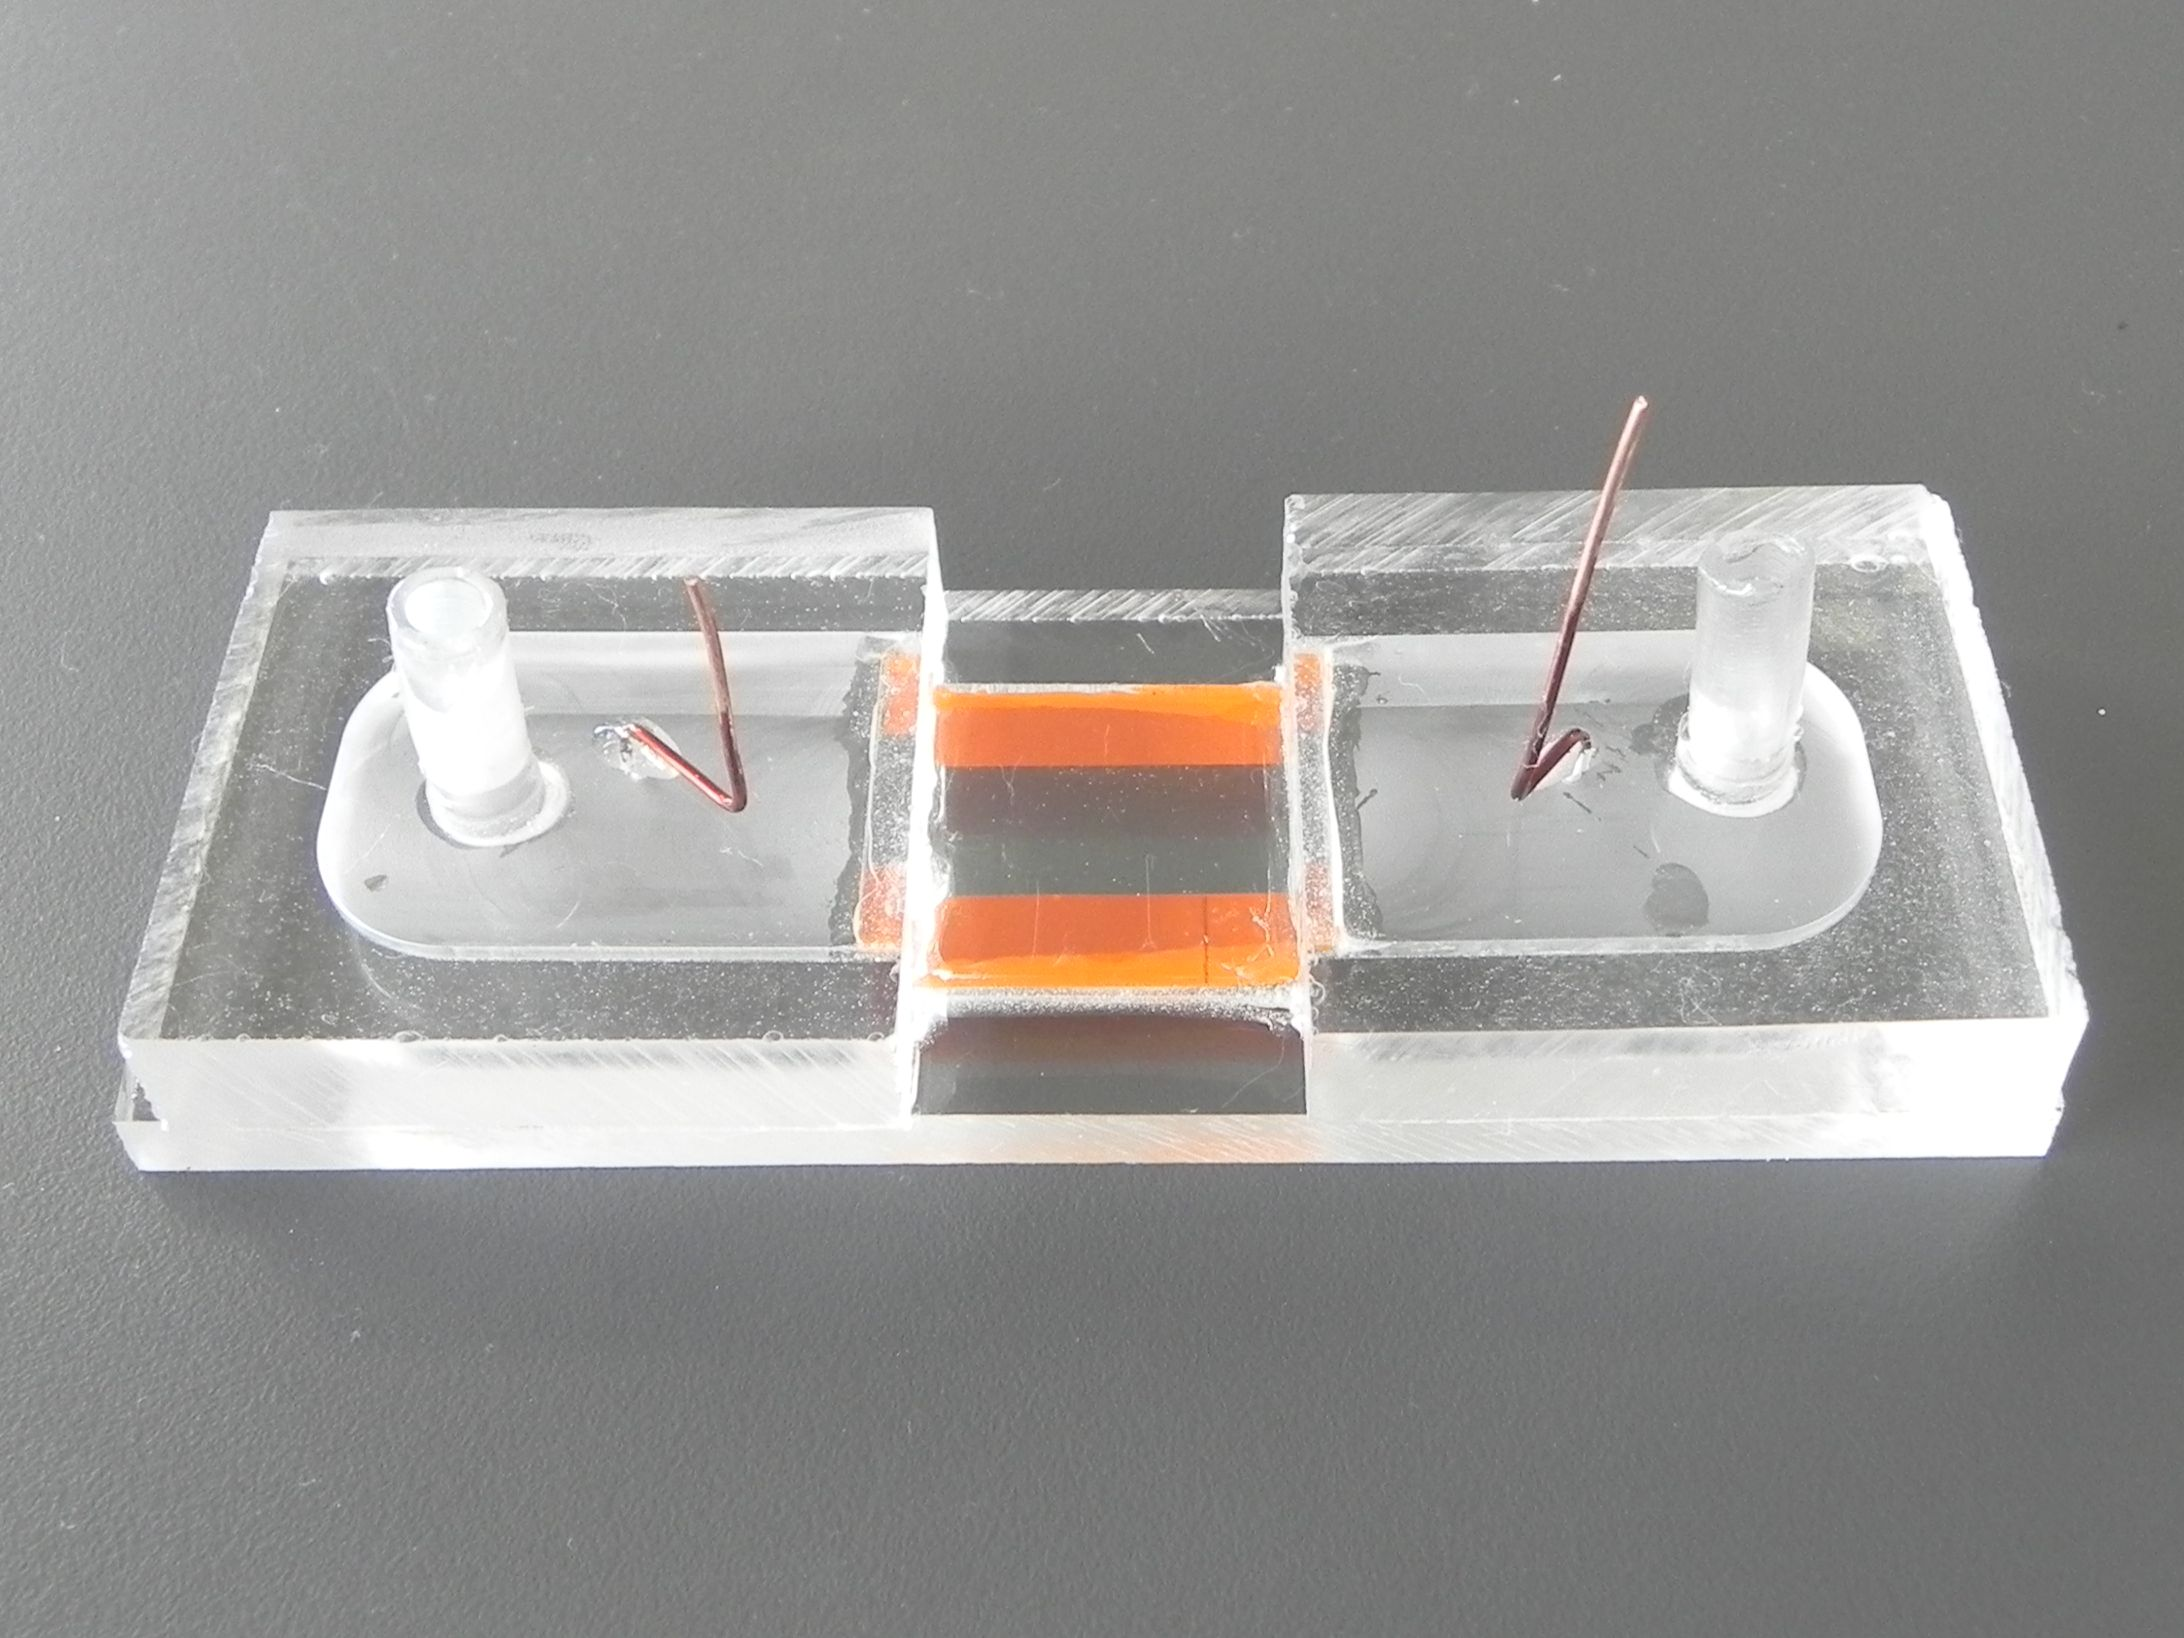
\includegraphics[width=\linewidth]{Photo_streamingPotential_Assembly_Step3.JPG}
        \end{center}
        \caption{One of ten constructed streaming cells mounted in an acrylic holder. Copper wires have been epoxied into each side to provide a means of measuring the developed potential across the cell. The shim is visible as the two orange strips at each side of the cell.}
        \label{fig:cell}
    \end{figure}
    A photo of one of the cells is shown in Fig. \ref{fig:cell}.

    \section{Estimation of Typical Household Water Consumption}
    \label{sect:waterConsumption}
    \section{Estimation of Power Requirements}
    \label{sect:powerRequirements}
    \section{Estimation of Streaming Cell Harvester}
    \label{sect:harvesterSize}
    \section{Conclusion}
    \bibliographystyle{plain}
    \bibliography{library}

\end{document}
